\begin{figure}[!ht]
 \centering
 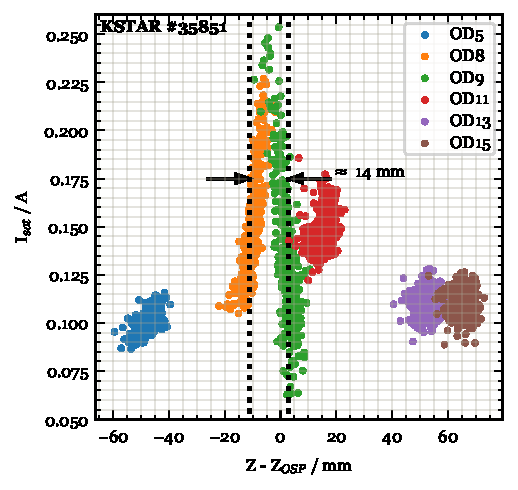
\includegraphics[width=\linewidth]{figures/StrikePointWidth.pdf}
 \caption{
Strike point width estimation for reference shot \#35851.
The raw data from langmuir probe array has been filtered by 4th order Butterworth filter with cut-off frequency of 20 Hz and then down sampled to 40 Hz.
For each data point on this plot, the x-axis position is calculated by subtracting the \ac{OSP} position reported by EFIT from the probe's Z coordinate.
The black dotted lines represent the rough estimate for width of strike point ion saturation current profile taken at half the maximum value above baseline.
}
 \label{fig:strike_point_width}
\end{figure}